\documentclass[useAMS,usenatbib]{mn2e}

\usepackage{epsfig}
\usepackage{epstopdf}
\usepackage{lscape} % Allows landscape environment to be used

\def\lesssim{\mathrel{\hbox{\rlap{\hbox{\lower4pt\hbox{$\sim$}}}\hbox{$<$}}}}
\def\gtrsim{\mathrel{\hbox{\rlap{\hbox{\lower4pt\hbox{$\sim$}}}\hbox{$>$}}}}
\addtolength{\topmargin}{-0.7in}

\title[Interstellar Plasma Scattering]{
Pulsar scintillations from corrugated reconnection sheets in the ISM
}
\author[Pen and Levin]{Ue-Li
  Pen,$^{1}$\thanks{E-mail:\ pen@cita.utoronto.ca}
Yuri Levin,$^2$\thanks{E-mail:\ yuri.levin@monash.edu}
}
\begin{document}


\date{\today}

\pagerange{\pageref{firstpage}--\pageref{lastpage}} 
\pubyear{2012}

\maketitle
\label{firstpage}
\begin{abstract}

We show that surface waves along interstellar current sheets closely
aligned with the line of sight lead to pulsar scintillation properties
consistent with those observed.  By contrast with previously
considered scintillation drivers, our mechanism naturally produces the
length and density scales of the ISM scattering lenses that are
required to explain the magnitude and dynamical spectrum of the
scintillations.  In our picture, the parts of warm ionized
interstellar medium that are responsible for the scintillations are
relatively quiescent, with scintillation and scattering resulting from
weak waves propagating along magnetic domain boundary current sheets,
which are both expected from helicity conservation and have been
observed in numerical simulations.  The model quantitatively predicts
the spacing and amplitudes of inverted parabolic arcs seen in
Fourier-transformed dynamical spectra of strongly scintillating
pulsars. Multi-frequency, multi-epoch low frequency VLBI observations
can quantitatively test this picture.  If successful, in addition to
mapping the ISM, this opens the door to precise nanoarcsecond pulsar
astrometry, distance measurements, and emission studies using these
10AU interferometers in the sky.
%THE LATEST STATEMENT IS CURRENTLY NOT BACKED UP BY ANYTHING IN THE PAPER.

\end{abstract}
\begin{keywords}
Interstellar Medium, reconnection
\end{keywords}

\newcommand{\be}{\begin{eqnarray}}
\newcommand{\ee}{\end{eqnarray}}
\newcommand{\beq}{\begin{equation}}
\newcommand{\eeq}{\end{equation}}

\section{Introduction: observations and theoretical challenges}

Compact radio sources provide a precision probe of the ionized interstellar medium
(IISM).  The propagation speed of radio waves depends on the density
of free electrons, and therefore the spatial inhomogeneity of the IISM may result in refractive and diffractive
abberation and scattering. This causes scintillation (time-variability) of the compact radio-sources
 \citep{1968Natur.218..920S,1986ApJ...301L..53B,2006ApJS..165..439R}. 
Observations of the pulsar scintillations are particularly interesting for infering the IISM properties, 
due to the brightness of many pulsars that have been observed for other purposes over long time intervals.

However, despite of considerable effort, the small-scale structure of the IISM
has remained enigmatic. At a first glance, one expects the scattering to be caused by density
inhomogeneities produced from turbulent motions of the IISM. However, this picture
is in contradiction with the last decade of the pulsar scintillation data.   There, a
major observational progress of the ISM scintillations has been
achieved through the \citet{2001ApJ...549L..97S}
detection of parabolic structures in the Fourier-transformed dynamical
spectra of strongly scintillating pulsars. These parabolic structures
imply that for these pulsars the radio-wave scattering occurs mostly
within one or several thin screens
\citep{2004MNRAS.354...43W,2006ApJ...637..346C,2008MNRAS.388.1214W}.
%Walker et al.~2004, Cordes etal.~2006, Walker et al.~2008)
Moreover, the multiple ``inverted
parabolae'' \citep{2005ApJ...619L.171H} show that the scattering
inside the screen is strongly inhomogeneous and occurs in
localized clumps. The latter was recently confirmed by \cite{2010ApJ...708..232B} who have obtained the VLBI scattering
image PSR B0834+06. They
have found that not only the scattering image was clumpy but that the
clumps lined up along a thin line.
All of these
observational facts present a major challenge for theoretical
interpretation where the scattering is caused by density inhomogeneities produced in a turbulent
cascade \citep{2001ApJ...562..279L}. In particular, (1) the origin of the screens is unexplained,
and (2) the strongly non-gaussian scattering requires AU-size
regions which are over-pressurized by factors of $\sim 10^3$
relative to the ambient warm ISM \citep{1987Natur.328..324R}; no conventional
physical mechanism has been proposed for how such regions may be
formed.

In this paper, we advocate a scenario in which the scattering is produced by a refractive structure, 
with turbulence playing a secondary role.
Radio-wave scattering by non-turbulent large-scale refractive structures has been previously
considered by Romani, Blandford, \& Cordes (1987), mostly in the context of the so-called
extreme-scattering events observed by
\cite{1987Natur.326..675F}. Recently, \cite{2006ApJ...640L.159G}
proposed that the image of the SgrA* radio-source is  
strongly scattered by several reconnection sheets that are closely aligned with the line of sight to
SgrA*.
In this paper, we develop further the Goldreich \& Sridhar's (2006) idea [see also \cite{2012MNRAS.421L.132P}] 
and apply it to construct a quantitative
picture of pulsar scintillations. Namely, we consider a scenario where
the pulsar radio-wave scattering occurs due to several {\it weakly corrugated} 
reconnection sheets that are
closely aligned with the line of sight to the pulsar; see figure \ref{fig:sheetgeom}.  We show that this scenario provides
compelling explanations for previously unexplained features of the scintillations: 
(1)  the ``scattering screens'' are simply effective descriptions of such sheets; their location is marked 
approximately
by the sheets' intersections with the line of sight, (2) ``the scattering clumps'' correspond to 
those parts of sheet folds where the sheet is parallel 
to
the line of sight; the strength of the scattering follows a strongly non-Gaussian distribution, even though
the corrugation itself is assumed to be a realization of a Gaussian distribution, and (3) the
strong non-isotropy of the Brisken et al.~2010 image is a consequence of the sheet's inclination, 
with the clump locations aligned along the direction perpendicular to sheet's line of nodes. The plan of the paper is
as follows: in the next section we briefly describe the origin of the
reconnection sheets, in section 3  we derive the model for the fold statistics,
in section 4 we derive the lensing by the corrugated sheet, and in section 5 we compute the
Fourier-transformed dynamical spectrum and demonstrate the parabolic structures. In section 6 we conclude.



\section{Astrophysical Picture}

\subsection{Two Regimes of Lensing: Diffractive vs Refractive}

Two regimes to generate pulsar scintillation have been considered. In
the diffractive regime, the scattering/lensing angle is determined by
the ratio of the wavelength
$\lambda$ of the radio-waves, and the characteristic spatial scale $L$ of the scattering structure: $\theta\sim\lambda/L$.   The brightness of the scattered
image  is determined by the amplitude of the wavefront modulation caused by the scattering structure.  To explain
the observed angles in the range $1-100$ mas at wavelength $\sim 1$m,
requires structures in the ISM on scales of order $10^{6-8}$m. This
imposes unexpected properties on the IISM, since this scale
much smaller than the coloumb mean free path of protons and thus compressive perturbations of
this scale are overdamped and decay esponentially on the sound-crossing time-scale.  If one still assumes that somehow these perturbations are created and maintained,
then the angular image of a
pulsar, and therefore its dynamic spectrum, are superpositions of
thousands of 
$\hbox{AU}/10^8\hbox{m}$ weak structures (for a 1-d scattering image),
and are expected to be roughly Gaussian.  The length scale is given by
the path length difference, which in turn is inferred from the
inverse scintillation correlation frequency.
The
parabolically structured 2-D power spectrum of the dynamic spectrum,
and the VLBI image of the scattering disk consisting of several prominent clumps, are inconsistent with such
a picture.  The number of $10^{6-8}$m eddies along the line of sight
can be large, possibly $10^{13}$ for a pulsar at a distance of $\sim$
kpc.  The total scattered power comes from the cumulative projected
variation in refractive index, which grows as the square root of the
number of eddies.  Each eddie only needs to change the refractive
index by a part in a million of the cumulative change, so a refractive
index variation of a part in $\sim 10^{12}$ could account for the
strong scintillation.   But the superposition of such a large number
of eddies would surely look very Gaussian from the central limit
theorem.  An intermittency of $10^{13}$ to appear intermittent in
projection would lead to highly overpressurized eddies.

A second mechanism is due to refractive lensing.  In this scenario,
the bending angle is determined by Snell's law, i.e. the change in
refractive index and the angles of incidence.  The refractive index of
a plasma is $n=1/\sqrt{1-\omega_p^2/\omega^2}$, with plasma frequency
$\omega_{\rm p}=\sqrt{n_e e^2/\epsilon_{0}m_e}$.  Pulsar observations
are done at frequencies much higher than the plasma frequency, for which
we expand $n-1 \sim \frac{\omega_p^2}{2 \omega^2} = 1.8\times 10^{-8}
n_e$ at wavelengths of a meter.  The observed scattered images at 20
mas require deflection 
angles of at least 40 mas, corresponding to $n_e \sim 10/{\rm cm}^3$ neglecting
geometric alignment factors.  However, the mean density of the IISM is
determined to be
of the order $10^{-2}$, as measured  from the pulsars' dispersion measure\citep{2004hpa..book.....L}.
%The flux of the images
%is determined by the size of the lens over the impact parameter. 
Therefore, the refractive picture is  also challenging to reconcile with the data, since the observed
scattering angles would na\"ively require fractional changes in free electron
density of $\sim 10^3$ 
which are difficult to understand or confine. This contraint, however, is alleviated
when one considers refractive sheets that are closely aligned with the line of sight
\citep{2006ApJ...640L.159G}.

Historically, refractive lensing was used to interpret long time
variability, and diffraction for the minute time scale
effects. Recently, it was understood that the refractive images result
in an interference fringe pattern \citep{2004MNRAS.354...43W} which have
similar time and frequency scales for flux modulation as diffractive
effects.  The frequency and time scaling was historically interpreted
as related to an underlying stochastic diffractive process driven by
turbulence.
\cite{2006ApJ...640L.159G} showed that refractive lensing by aligned
sheets  results in
scintillation similar to the diffractive picture.




%!!The discovery of parabolic arcs\citep{2001ApJ...549L..97S} and
%inverted arclets has required the existence of localized refractive
%lenses.  Direct VLBI imaging of the scattering
%screen\citep{2010ApJ...708..232B} demonstrate the presence of
%discrete isolated lenses, i.e. scattering points, which are all in a
%single thin sheet. This leads to physical challenges of confining
%these lenses. Various solutions have been
%proposed\citep{2007ASPC..365..299W,2012MNRAS.421L.132P,2006ApJ...640L.159G}.

%In this paper, we expand the picture of current sheets, and consider
%perturbations.!!


\subsection{Physical origin of the reconnection sheets}

The interstellar medium is stirred on scales of parsecs by various
energetic processes, including supernovae, ionization fronts, spiral
density waves, and other phenomena.  These processes are generally
short lived, and we conjecture after the stirring, the warm medium
relaxes to an near-equilibrium configuration on small (several AU)
scales. Current numerical simulations of the supernova-driven
turbulence in the warm ISM of the Galaxy (e.g., Hill et al.~2011) do
not have the resolution to tell how realistic this assumption is.  In
the presence of helicity, the equilibrium magnetic fields are
configured as interlaced twisted tori, which are long lived
\citep{2004Natur.431..819B}.  It has been shown by \cite{2009arXiv0909.1815G}
that a ``generic magnetic equilibrium of an ideally conducting fluid
contains a volume-filling set of singular current layers.'' In this
picture, the magnetic fields are locally almost parallel, with
discontinuous interface regions, a bit like magnetic domains in a
ferromagnet. Singular current sheets have also been seen in the
simulations of \citet{2004PhRvL..92h4504S}.

At the boundary between between magnetic field configurations, current
sheets maintain the discontinuities.  Depending on the nature of
reconnection, these current sheet may be self-enforcing due to inflow
of fresh fields, maintaining a thickness potentially as thin as an
electron gyromagnetic radius.  At constant temperature,
the pressure equilibrium in the direction
perpendicular to the sheet implies that the electron density inside the sheet is
enhanced by a factor $R$ given by
\begin{equation} 
R-1\sim {B_{\rm out}^2-B_{\rm in}^2\over 4\pi P_{\rm out}},
\label{ratio}
\end{equation}
  where $B_{\rm in}$ and $B_{rm out}$ is the magnetic field in and outside the sheet,
  and $P_{\rm out}$ is the non-magnetic pressure outside the sheet. The right-hand side of
  the above equation is thought to be of order $1$ for the IISM, but may be significantly
  larger if the IISM is magnetic-pressure dominated. 

Depending on the ratio of heating time due to reconnection to cooling
time, the thin sheet may have an enhanced temperature, in which case
it can be underdense, with $R \rightarrow 0$ in the limit of a
strong entropy injection.


  %These current sheets have been
%proposed to dominate the scattering of radio
%sources \citep{2006ApJ...640L.159G}.

\begin{figure*}
\centerline{\epsfig{file=sheetgeom.eps,width=7.5in}}
\vspace{-6in}
\caption{lensing geometry.  The earth is at left, pulsar at right.
A section of the scattering sheet is in the middle.  The dashed line 
shows the  unperturbed light path.  The dotted line shows the path of 
an image
lensed by a fold caustic of the projected sheet.}
\label{fig:sheetgeom}
\end{figure*}

The lensing geometry is shown in Figure \ref{fig:sheetgeom}. A crucial ingredient in our model
is that the reconnection sheet is assumed to be weakly corrugated. Let is assume that the corrugation
pattern is fixed, and vary the inclination angle. In this case, as can be seen from 
figure \ref{fig:sheetgeom},
there is characteristic inclination angle $\alpha$ at which the perturbations in the
sheet can generate caustics in the projected surface density.  This
angle $\alpha$ is the ratio of the wave peak displacement to its
wavelength.  We envision ranges of $\alpha \sim 10^{-3} - 10^{-2}$.
When the caustics are present, they
become effective refractive scattering centers for the radio waves. The resulting lense features
multiple images that closely line up along the direction perpendicular to the line of nodes of the
scattering sheet.


\subsection{Surface Dynamics}

We assume that the current sheet is physically thin, $\lesssim $ AU.  Theoretically,
the thickness of current sheets is not understood, so we choose this
scale to be thin enough to explain the smallest scale observed
structures.  On each side the
magnetic field points in a different direction.  The change in alvenic
properties gives rise to surface
waves \citep{1991SoPh..133..263J, 2009GApFD.103...89J}, whose amplitude
decays exponentially with the distance to the current sheet and which are
mathematically analogous to deep water ocean waves.  The restoring force is due to the
difference in magnetic field component projected along the wave
vector.  Like ocean waves, these waves penetrate about a wavelength
into each side.  We will be considering wavelengths of hundreds to thousands of
AU whose projected wavelength is related to the observed lensing
structures  $\sim$several AU, so the thickness of the current sheet itself is
neglible as far as the dynamics of 
the waves are concerned.  Seen in projection along the aligned sheet,
the projected wavelengths will be $\sim $ AU, reduced by the alignment
angle $\alpha$.

The displacements are
transverse to the wave vector, and perpendicular to the sheet.  While
alvenic in nature, the surface modes possess only one polarization,
unlike bulk waves.  These waves resemble a flag blowing in the wind.
Disturbances travelling along the sheet are decoupled from bulk waves.
Being confined to a sheet, the amplitude away from a source drops as
$\propto 1/r$ instead of the normal inverse square law.  A amplitude
of order $\alpha \lambda_{\rm wave}$,   or about $10^{-3}$--$10^{-2}$ of the wavelength
of the surface wave, is
sufficient to cause the sheet to appear folded in projection; here $\lambda_{\rm wave}$ is the wavelength of the surface wave.

%\subsection{Sheet statistics}

%Here we consider the lensing effect of a large ensemble of sheets.  To
%understand the qualitative statistical behaviour, we consider
%infinitely thin round sheets, with one dimensional density
%corrugations on each sheet.  This problem is effectively one dimensional.
%THIS PART IS NOT DONE, TO BE REMOVED RIGHT?

\section{Fold Statistics}

%Alven waves dissipate on scales shorter than the proton mean free
%path THEY DON'T ACTUALLY; SEE BARNES Phys. Fluids 9, 1483 (1966).  

We expect a minimum wavelength of these surface waves, which is
substantially larger than the thickness of the sheet.  Short
wavelength perturbations are not bound to the surface, and can
dissipate into the bulk.  The exact cutoff depends on unknown factors,
including the distance to the source, and vertical structure of the
current sheet.  Non-linear effects also cause short wavelength waves
to dissipate, just like sound waves in the air.  Primarily waves with
amplitude larger than $\alpha$ contribute to scattering.  The strength
of damping depends on the distance to the source in units of
wavelength, with shorter wavelengths being more damped.


We model the waves as a displacement function $\zeta(x)$
which is a Gaussian random field with a correlation function that is a
Gaussian, 
\begin{equation}
\xi(r)=\langle \zeta(x)
\zeta(x+r)\rangle=A^2\exp\left(-{r^2\over 2\sigma^2}\right),
\end{equation}
where $A$ is the mean amplitude
of the displacement and $\sigma$ is the surface-wave
coherence scale.  Figure \ref{fig:sheet} shows a realization of a
sheet with a random fluctuations.  We used an inclination slope
$\alpha=1/8$, and a correlation length along the sheet of 350 units,
which is $\sigma_y\sim 44$ grid units in projection.  The displacement
amplitude is chosen as $A=40$.  The dimensionless fluctuation
$\delta\equiv A/\sigma \sim 1$ is about unity, meaning a $1-\sigma$
flucuation can result in a caustic fold, which we will discuss further
below.

\begin{figure}
\vspace{-0.8in}
\centerline{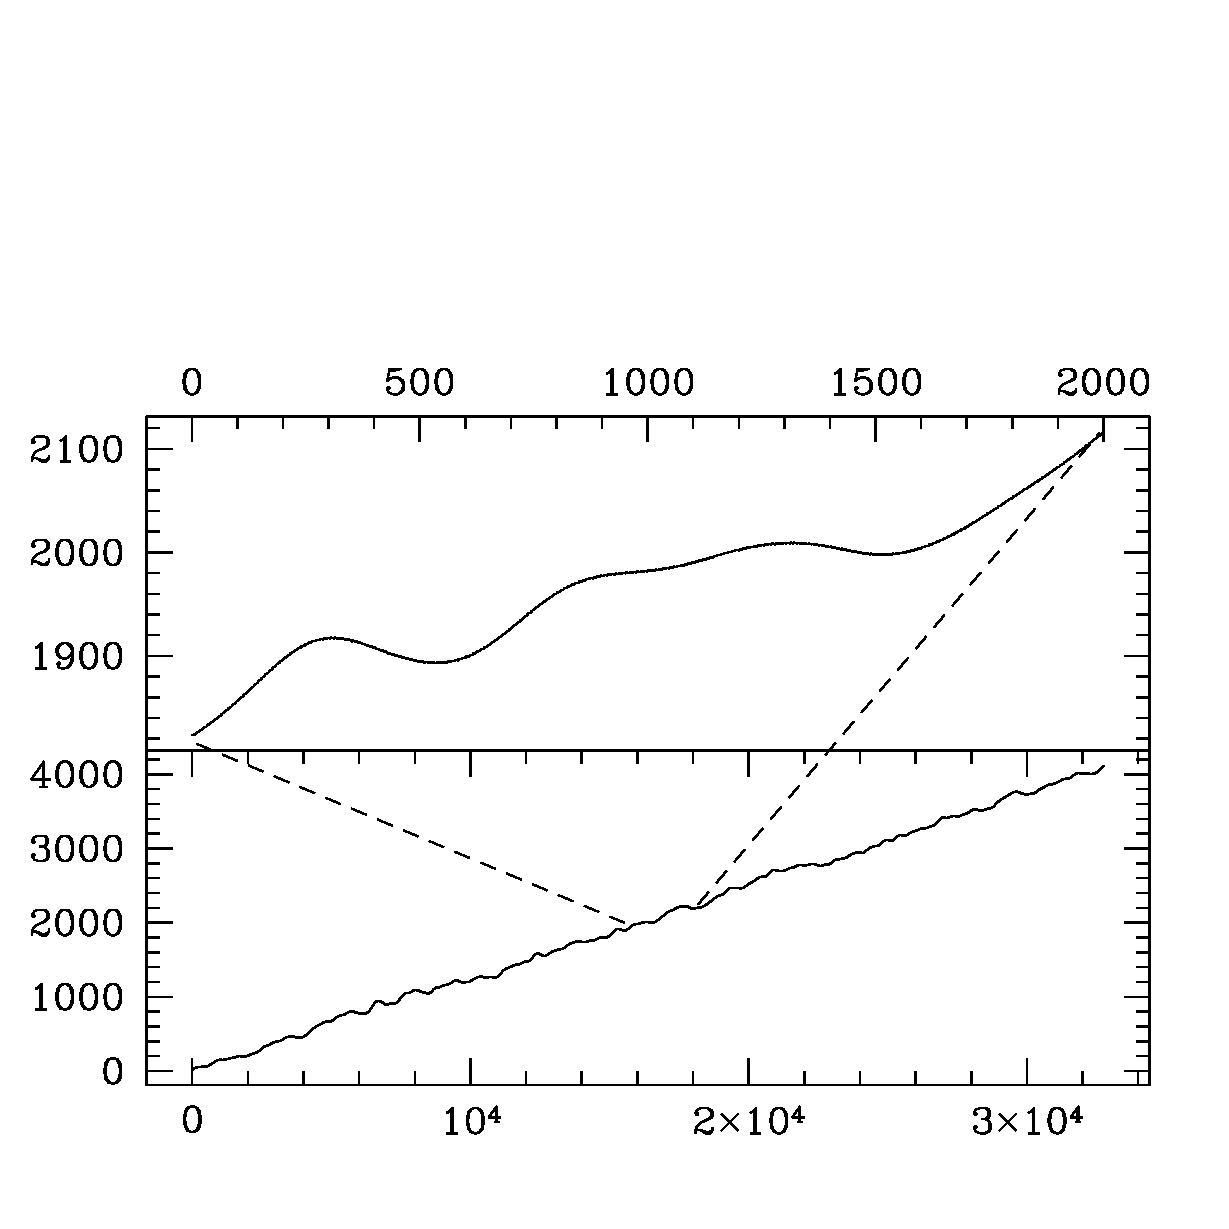
\epsfig{file=sheetz.eps,width=3in}}
\caption{Sheet with transverse perturbations.  The upper panel shows
  an zoomed version of a short section.}
\label{fig:sheet}
\end{figure}

The current sheet has a reduced magnetic pressure and thus has a refractive index different
from the ambient ISM. For simplicity, we assume here that the sheet has constant thickness, and
consider its optical depth as is relevant for refractive lensing.
In projection along the line of sight, the column density of the  sheet 
results in a highly non-Gaussian
distribution. Figure \ref{fig:rho} shows the column density distribution in a
simulation.  Folds occur when the gradient of the displacement is
equal to $-\alpha$, which as described above is quantified by the
fluctuation amplitude $\delta$.  The value chosen here makes folds
common, occuring roughly once per correlation length, and yet make
multiple folds overlapping in projection rare.  Each fold results in
two caustics, with characteric separation $\sigma_y$. This is well
understood from the theory of extrema of surface
waves\citep{1957RSPTA.249..321L}. 

%The correlation function of the gradients is the
%second derivative of the displacements.  The number of crossings of -1
%depends on the variance of the gradient field.  The density of the
%folded sheet is proportionate to the length of gradient spent in the
%vicinity of -1, which is turn is proportionate to the reciprocal of
%the derivative of the gradient.  This second derivative is also a
%Gaussian random field.  The second derivative is uncorrelated with the
%first derivative.  The one point PDF of the reciprocal of a Gaussian
%variable is
%\beq
%P(\rho)=\frac{\exp(-\frac{1}{2 \rho^2})}{\sqrt{2\pi}\rho^2}.
%\eeq
%UE-LI, I GET A DIFFERENT ANSWER. I DON'T HAVE THE FULL EXPRESSION, BUT 
%ASYMPTOTICALLY THE HIGH-END TAIL IS CLEAR. 
%
% 
% LET $\theta$ BE THE ANGLE BETWEEN THE 
As before,  $\alpha$ is the angle between the screen and the line of sight.
Then the optical depth is $\rho\propto1/\alpha$ for
$\alpha\ll 1$, and  $P_{\rm screen}(\rho)\propto 1/\rho^2$, where $P_{screen}(\rho)$
is the probability of a piece of screen to have the optical depth of $\rho$.
However, we are interested in the probability density with respect to the impact parameter relative
to the line of sight, and not with respect to the location on the screen. For nearly aligned screens, this
is not the same thing. In particular, part of the screen with low $\alpha$ occupies less of the
impact-parameter space than the part of the screen with the same area but high $\alpha$. Thus,
\begin{equation}
P_{\rm impact parameter}(\rho)\propto 1/\rho^3
\label{eqn:prho}
\end{equation}
which is a strongly non-Gaussian distribution.

\begin{figure}
\centerline{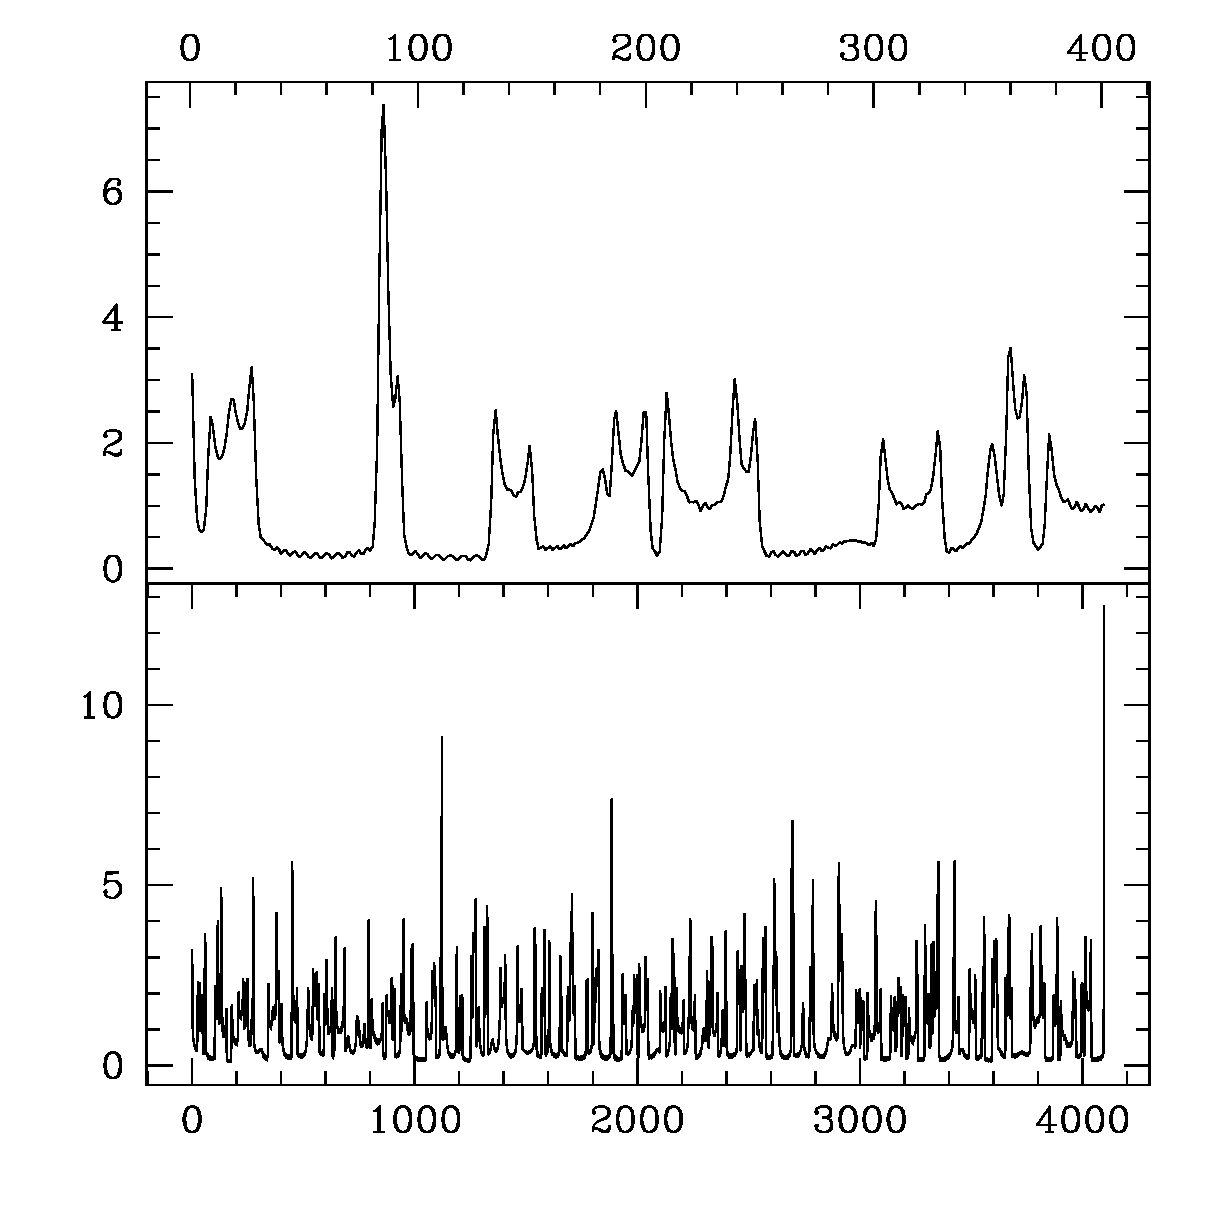
\epsfig{file=rho.eps,width=3in}}
\caption{projected density.  The upper panel is a zoom of the central
  portion of the lower panel. Each time the sheet folds in projection,
we see a double peaked caustic structure in density.  The
characteristic separation
between the two peaks is a projection correlation length $\sigma_y$,
in this case 44 grid units.}
\label{fig:rho}
\end{figure}

Equation (\ref{eqn:prho}) describes the 1 point PDF in figure
\ref{fig:rho}.  The deflection angle is the gradient of the density, $\rho'$.

As in \cite{2012MNRAS.421L.132P}, we use the notation of gravitational
lensing.  The convergence $\kappa \propto \rho''$ is given by the
second derivative of the density.  The magnification gives the
brightness of the image.  In 1-D it is $\mu=1/(1-2\kappa)$, derived
from the determinant of the amplification matrix.  A negative
amplification is a flipped image of odd parity.

The regions near the locations where the screen is parallel to the
line-of-sight, which the call the caustics, give rise to the localized
clumps in the pulsar's scattering image, which produce the inverted
parabolic arcs in pulsar secondary spectra.

\section{Lensing}

The lensing of this density sheet can be computed in analogy to 
 \cite{2012MNRAS.421L.132P}.

\begin{figure}
\centerline{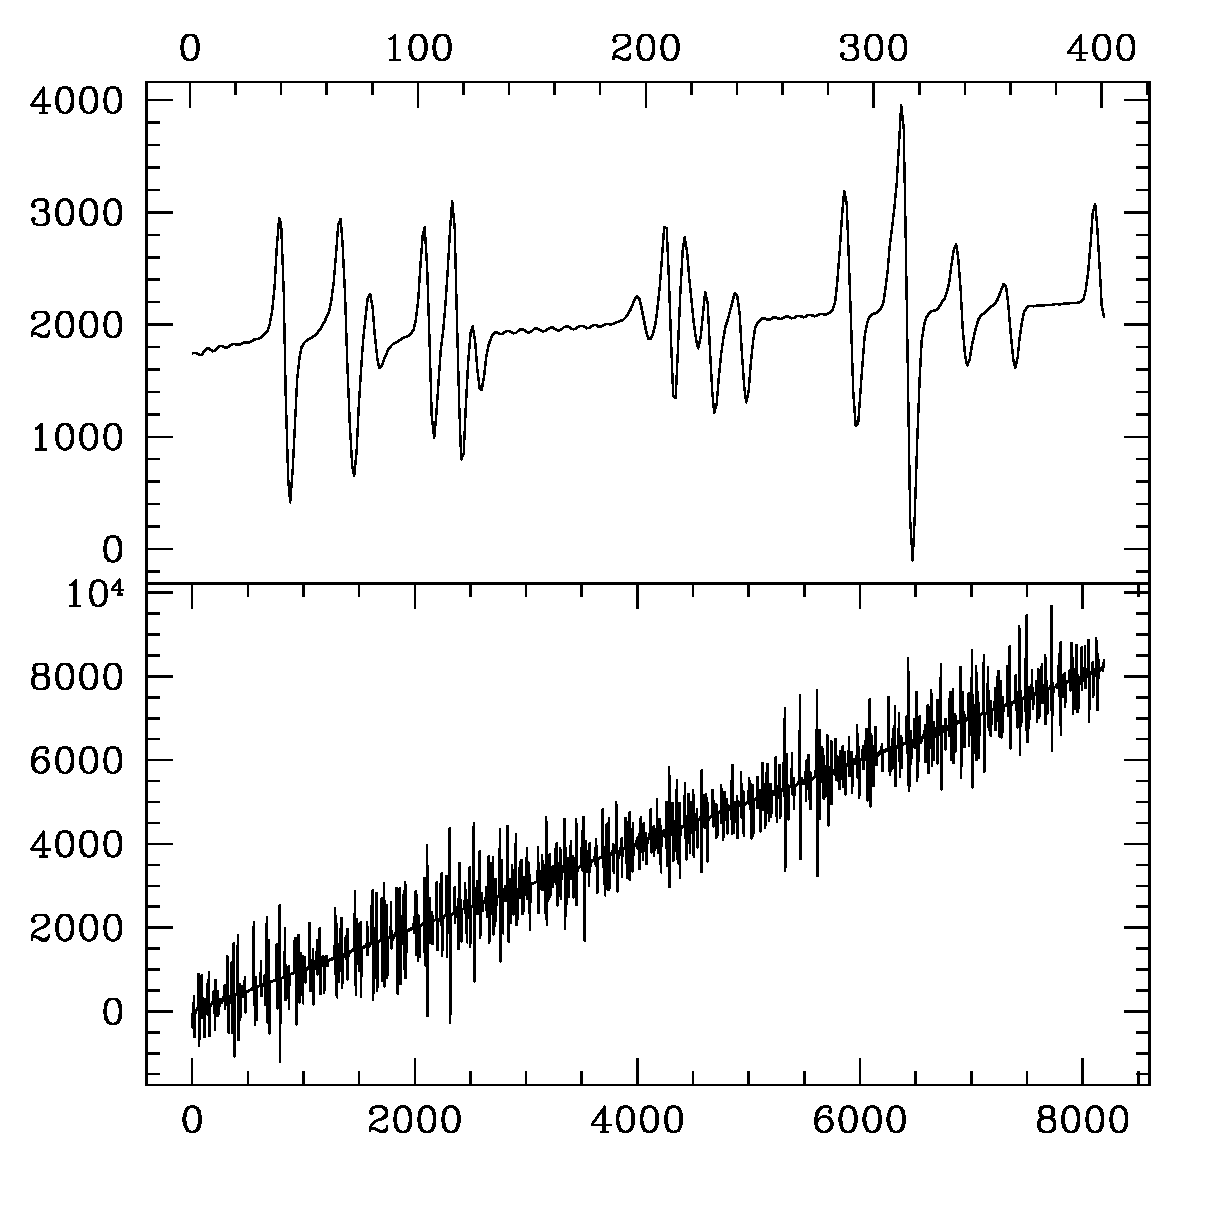
\epsfig{file=dt.eps,width=3in}}
\caption{deflection angle mapping. The horizontal axis is angle on the
sky, and the vertical axis is the intersection of this light ray on
the source plane.  Whenever multiple different directions on the sky
intersect on the same position in the source plane, multiple images
are formed, which form a coherent interference pattern.}
\label{fig:dt}
\end{figure}

Given the projected column density distribution in Figure \ref{fig:rho}, and assuming that
the sheet has a fixed optical depth along its normal, we
can compute the mapping of apparent angle on the sky to position in the
source (pulsar) plane.  The caustics in the projected density
distribution lead to large angle deflections, and multiple images,
whenever the sheets are aligned closely enough for the caustics to form.
This explains why only a small fraction of the current
sheets contribute to scintillation. 

The system depends on the dimensionless parameter $\delta$, the ratio $r$
of sheet thickness $z$ to the projected correlation length $\sigma_y$,
and the ratio of index of refraction change to the angular size of the
projection correlation length.

The model predicts the number density of images and their fluxes as a
function of their angular separation from the line of sight (and
therefore as the function of time lag).  It has a small number of
dimensionless parameters: $\delta,\ r,\ C$.


%THIS SEEMS LIKE A VERY STRONG
%STATEMENT, I AM NOT AT ALL SURE ITS TRUE.  

There is a
dimensional scaling of time units, which is a function of pulsar
transverse velocity, projected screen size, and observing frequency.
This is generally parameterized as the DISS time scale, $t_{\rm DISS}
\sim (\lambda/D) (L/v)$ where $D$ is the size of the lensing region,
$L$ is the distance to the pulsar, $\lambda$ is the observing
wavelength, and $v$ is the pulsar transverse velocity.  Note that in
this model, the lensing is refractive, sharing the time scales from
diffractive models, but none of the physics.

%IF WE MAKE
%THIS STATEMENT, WE NEED TO GIVE AN EXACT EXPRESSION, OTHERWISE OMIT
%IT.


We show a histogram of image magnifications in Figure \ref{fig:mhist},
which can be compared to holographic flux measurements
\citep{2008MNRAS.388.1214W}. The lensed images correspond to the
inverted arclets seen in secondary spectra.  The model predicts the
number of images as a function of separation, shown in figure
\ref{fig:pos}.


%DID WE NOT SAY THIS ABOVE?


%THIS FIGURE
%HAS NO UNITS ON THE X-AXIS. THE SAME GOES FOR FIGURE 7
% fixed: the caption describes the units now.

\begin{figure}
\centerline{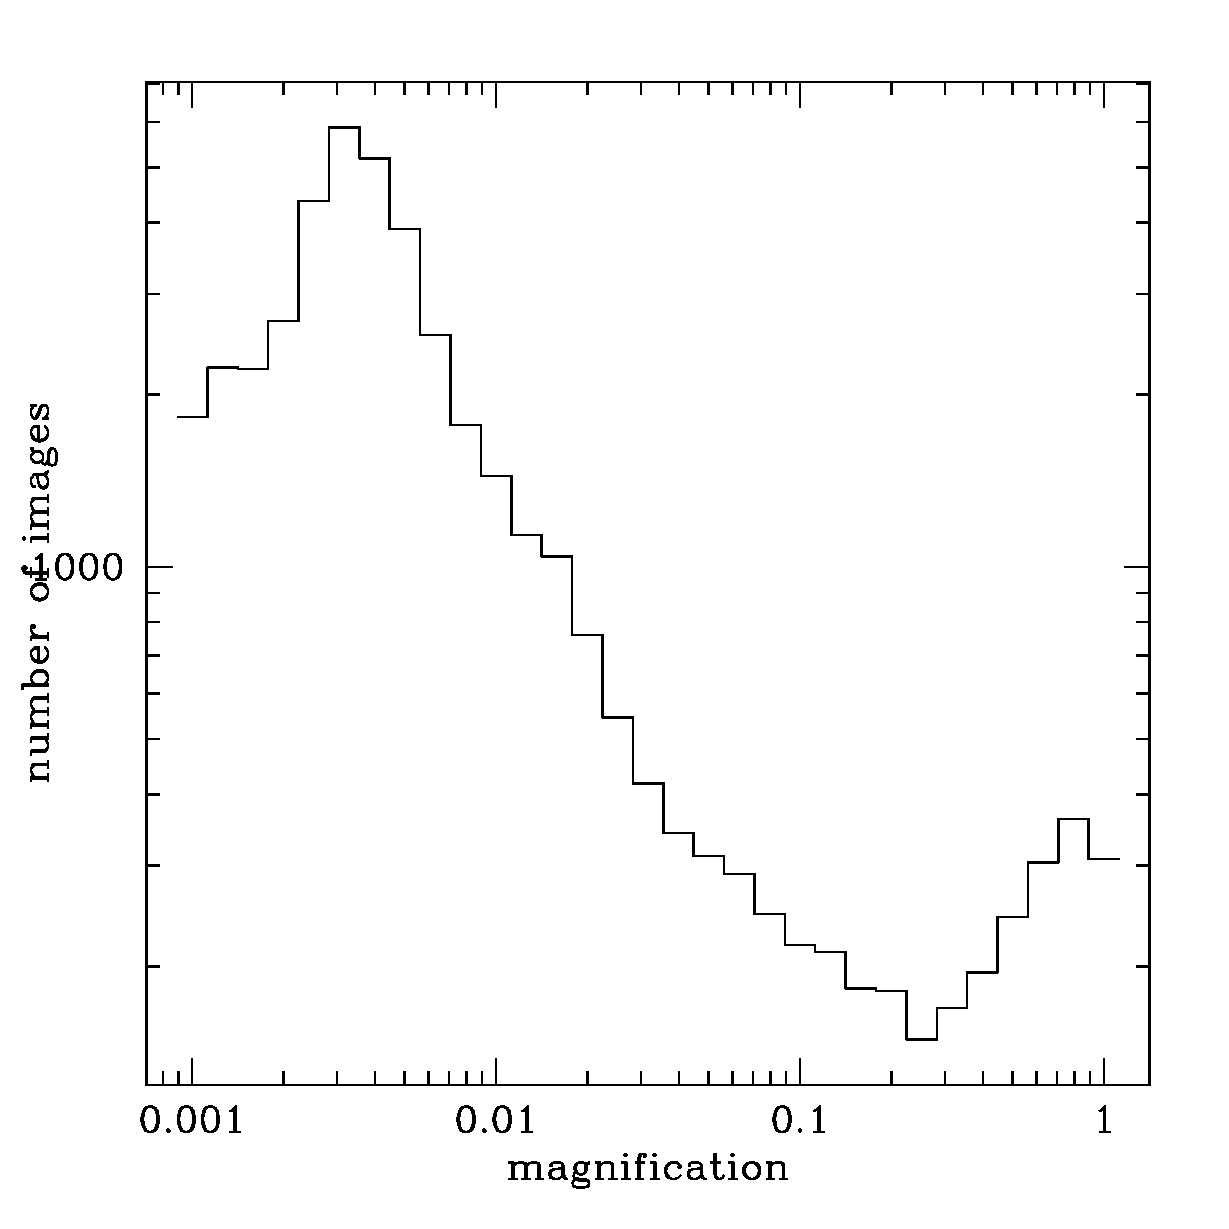
\epsfig{file=mag.eps,width=3in}}
\caption{PDF of image magnifications.  The peak near 1 are images at
  the unscattered positions, while the population on the left are
  lensed images.  The peak occurs at roughly $1/\kappa$.
}
\label{fig:mhist}
\end{figure}


The separation of images is related to the separation of caustics.
For the ``common'' limit of our simulation, $\delta \sim 1$, this is
given by the projection correlation length $\sigma_y$.  For $\delta \ll
1$, the caustics become very rare, proportionate to an error
function.   

\begin{figure}
\centerline{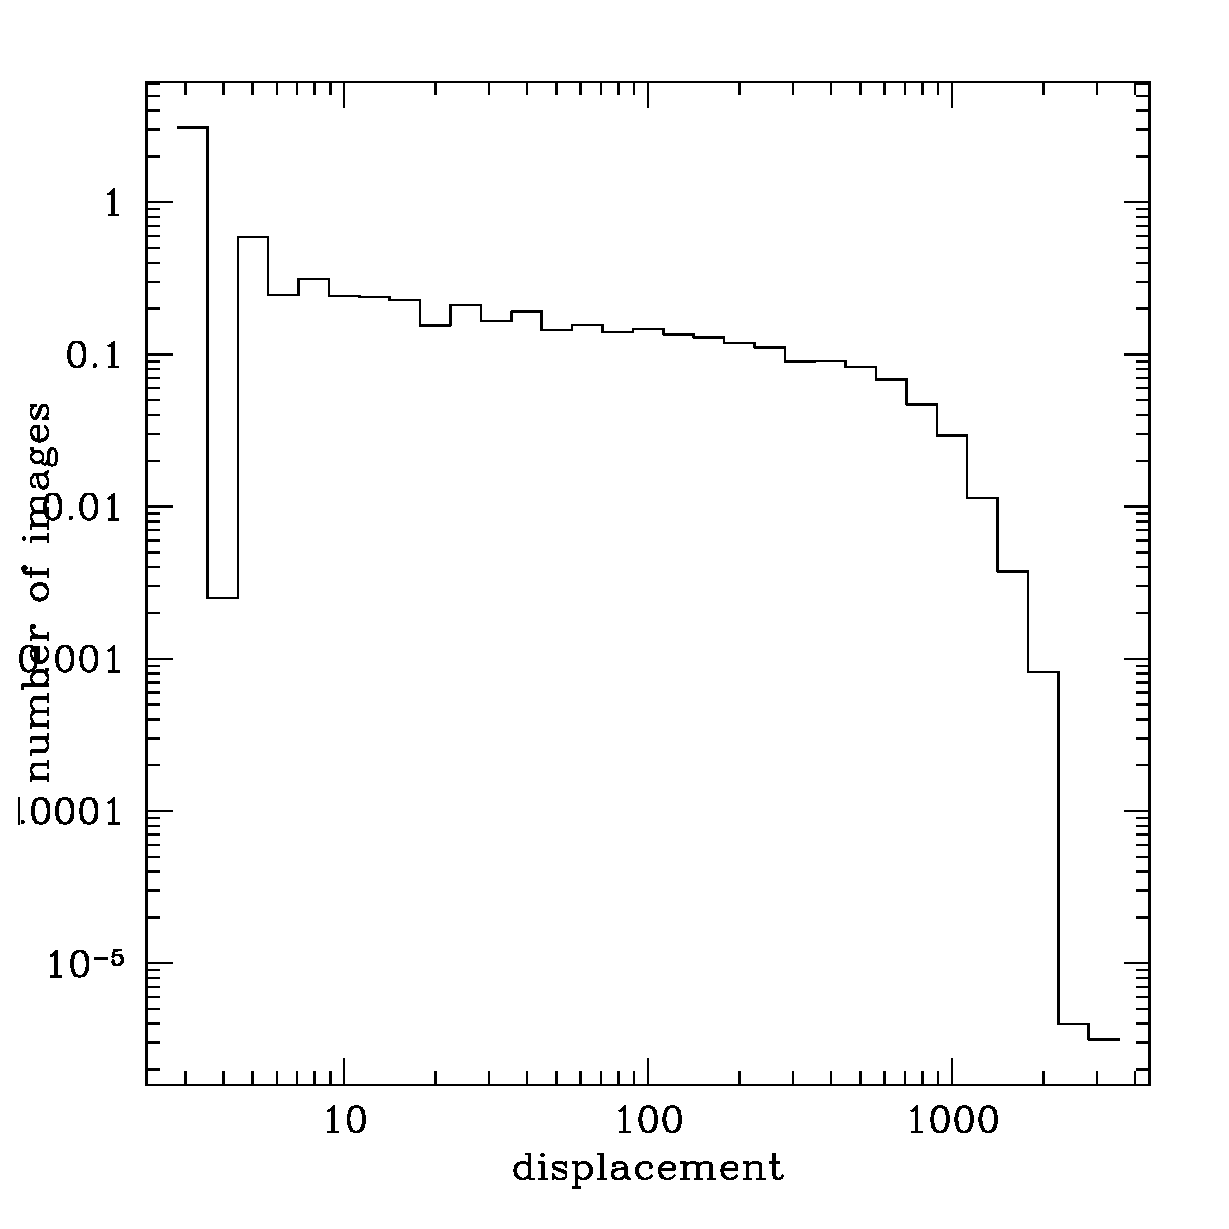
\epsfig{file=pos.eps,width=3in}}
\caption{PDF of image positions per logarithmic distance interval on
  the sky $y$.  The projected correlation length is $\sigma_y \sim
  44$.  The characteristic convergence $\kappa \sim 20$, leading to a
  cutoff near $\sigma_y \kappa \sim 1000$.
}
\label{fig:pos}
\end{figure}

The number of images is determined by the number of light folds along
the line of sight, i.e. how often the deflection angle is larger than
the separation to the line of sight in Figure \ref{fig:dt}.

\begin{figure}
\centerline{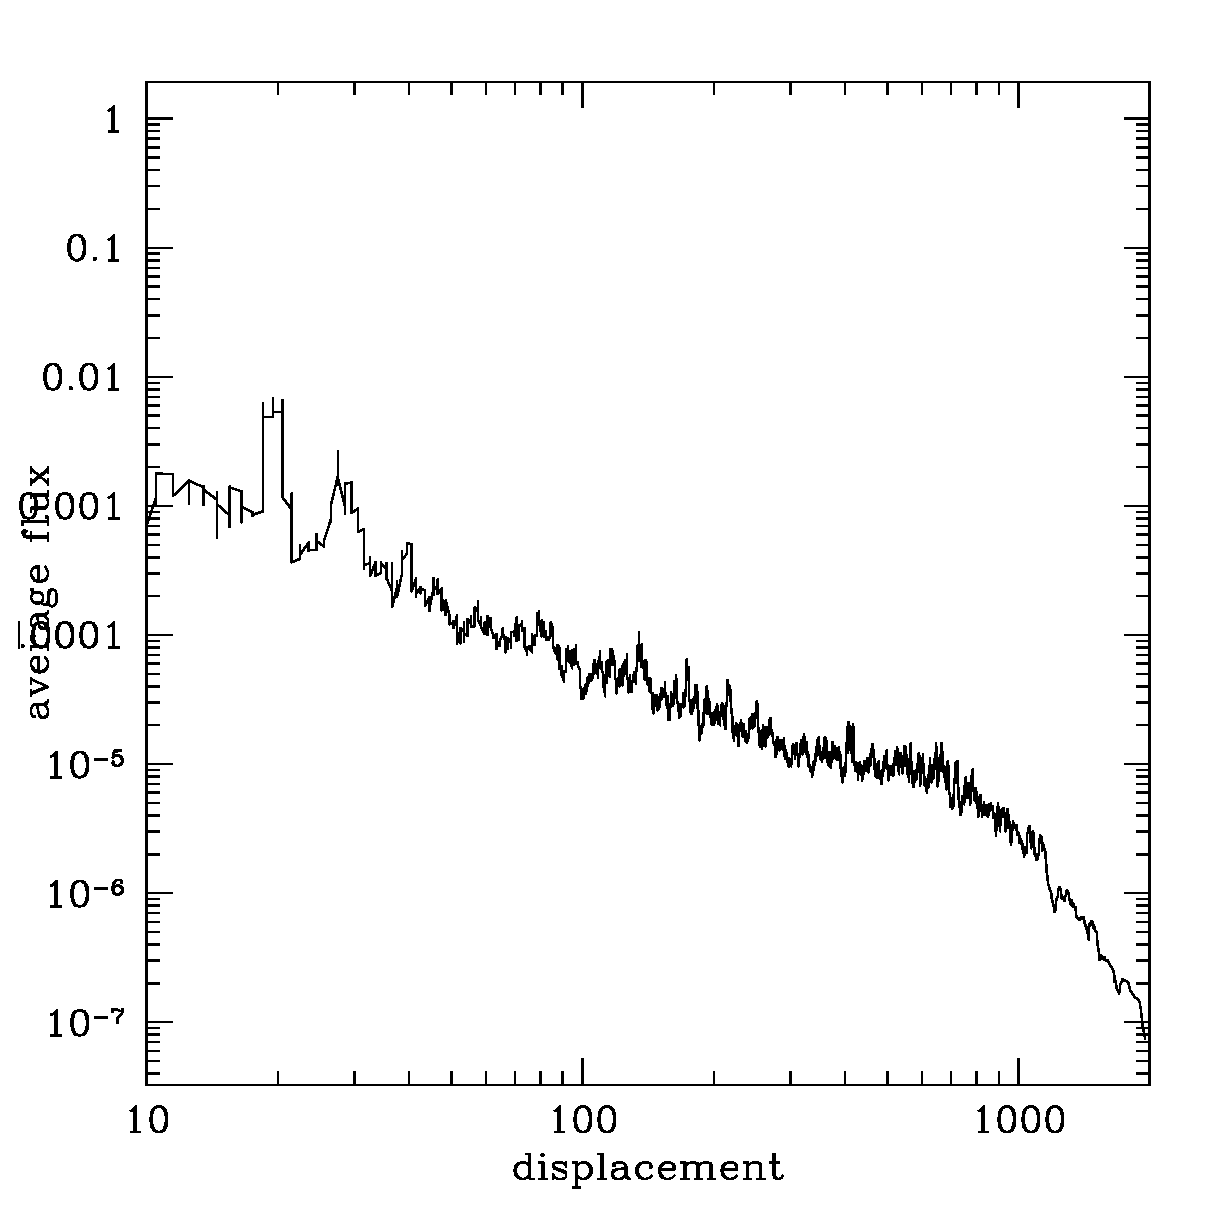
\epsfig{file=posmag.eps,width=3in}}
\caption{Average Spatial Distribution of flux per logarithmic distance
  interval.  In a Gaussian model, the flux per image drops as
  $1/\theta$. 
}
\label{fig:posmag}
\end{figure}

The maximum deflection angle of an image is the change of refractive
index in the sheet, amplified by the alignment angle on a fold
caustic.  For a sheet much thinner than the projected fluctation
amplitude, the maximum projected density enhancement $C$ at a caustic
is the square root of the radius of curvature to the thickness of the
sheet $\tau$, $C=\sigma/\sqrt{A\tau}$ in the limit $A \gg \tau$.
Much larger enhancements can occur for fluctuations comparable to the
thickness: at alignment angles $\alpha \sim A/\sigma$, the
enhancements can reach $C \sim 1/\alpha$.

\section{Simulated Dynamic Spectra}

With the density field, we can solve the lens equations to simulate
dynamic spectra.  By adding the voltages on each image  with their
appropriate amplitude and phases, we simulate the dynamic spectrum,
shown in figure \ref{fig:ds}.

\begin{figure}
\centerline{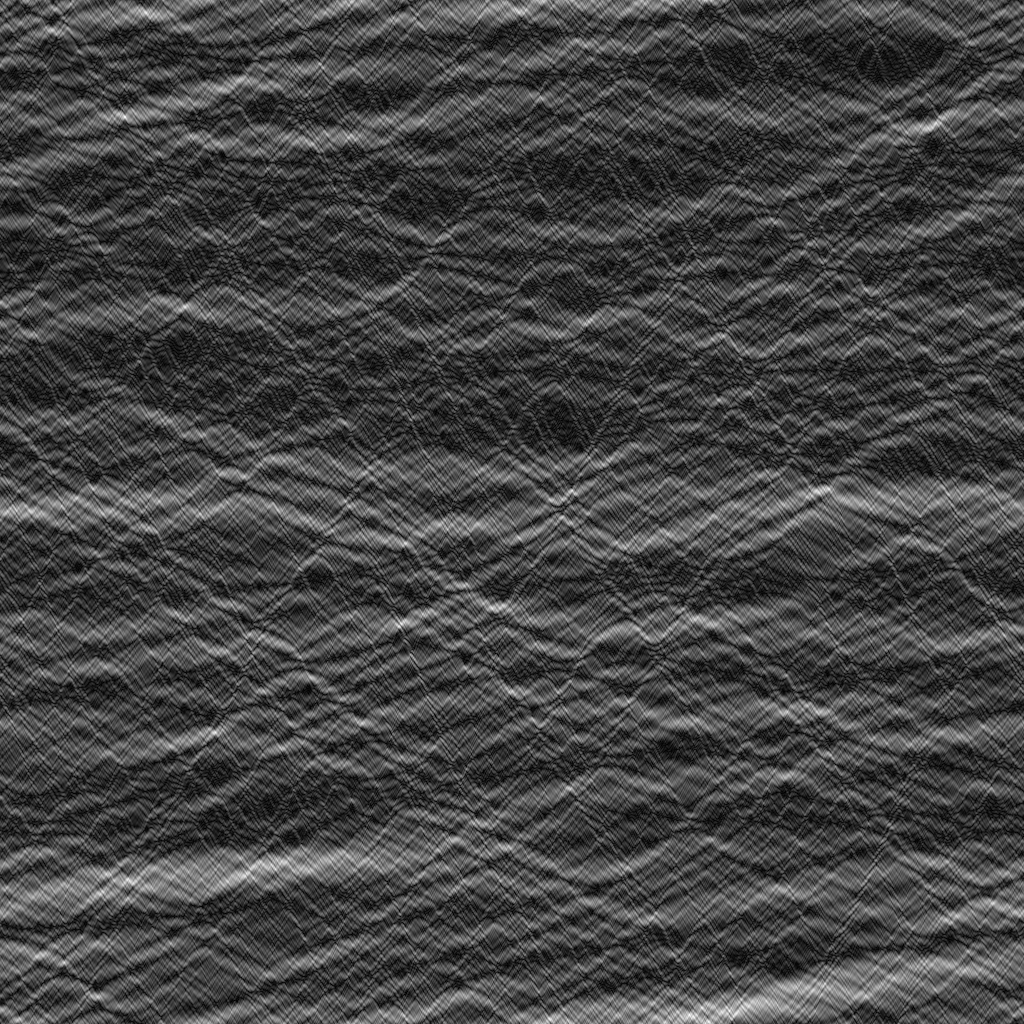
\includegraphics[width=3.5in]{rspect.jpg}}
\caption{dynamic pulsar spectrum.  Horizontal axis is time, vertical
  axis is frequency.  We reproduce the characteristic criss-cross
  pattern observed in real scintillation spectra.}
\label{fig:ds}
\end{figure}

A 2-D fourier transform maps this dynamic spectrum into a secondary
spectrum, shown in figure \ref{fig:ss}.

\begin{figure}
\centerline{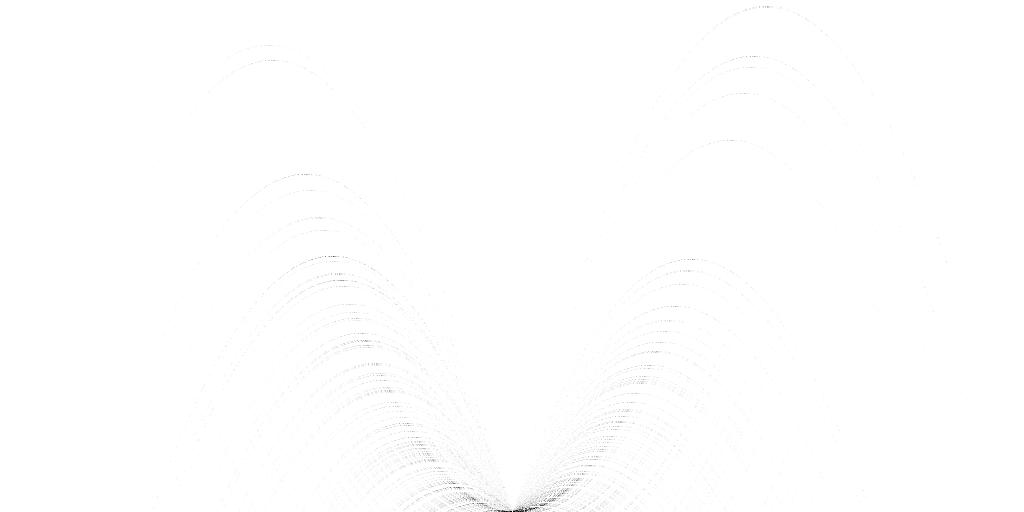
\includegraphics[width=3.5in]{sspectr.jpg}}
\caption{secondary pulsar spectrum.  The inverted parabolic arcs arise
naturally in this model.}
\label{fig:ss}
\end{figure}

We find that the interference of these discrete, co-linear images
forms the inverted parabolic arcs, qualitatively similar to those that are observed in
Stinebring et al.~(2001) and Hill et al.~(2005).



\section{Discussion}

We can estimate the length scales involved in making the current sheet that
would produce the observed scintillation pattern.  This theory requires as
input a current sheet thickness, inclination angle, curvature,
amplitude of waves, and dissipation scale.

The thickness of the sheets can be estimated by considering the magnification of
images.  As shown in \cite{2012MNRAS.421L.132P}, the flux is roughly
the thickness divided by the impact parameter.  This follows from flux
conservation of lensing: the net flux is conserved, and flux changes
by order unity at impact parameters of order the physical size of the
lens, so the typical flux off-axis is roughly the ratio of the
furthest distance at which at image forms, to the size the lens.  The
caustic itself only contains a small fraction of the integrated flux.


% WHY? NOT OBVIOUS TO READERS LIKE ME.  
The projected wavelengths
are observed to be of order $\sim 10$ AU;
this suggests a typical thickness of $h\lesssim 0.1$AU to explain the
$\sim$\%  scattering intensities observed in \cite{2010ApJ...708..232B}.
%AU WE SHOULD QUOTE SOME
%OBSERVATIONAL PAPER WHERE THESE MAGNIFICTIONS ARE MEASURED.  

%A wave
%of projected wavelength $\alpha \lambda_{\rm wave}$ enhances projected densities
%by a factor $w=\sqrt{\alpha\lambda_{\rm wave}/h}\sim 100$.  

The largest observed deflection angles at meter wavelength are $\gamma
\sim 0.01$", which requires an electron density change $\delta n_e\sim
100/C$ cm$^{-3}$.  For a typical interstellar plasma density of $n_e
\sim 0.03$, we need an enhancement factor $C\sim 3000$, which is
achieved at an alignment $\alpha \sim 1/C$ of about an arc minute,
with fluctuation amplitude $A\sim 0.1$ AU and a wavelength of $\lambda
\sim 1000$ AU.  This combination is not unique.

%UE-LI, I AM NOT SURE WHY YOUR PROJECTED ELECTRON DENSITY IS MEASURES
%IN CM$^-3$ AND NOT $CM^-2$. BUT IN ANY CASE LETS AGREE ON THE
%EXPRESSION FOR THE LARGEST DEFLECTION ANGLE. I GET $\gamma'sim \delta
%n_e w/\alpha$. SEE IF YOU AGREE WITH THIS.

As discussed in \cite{2012MNRAS.421L.132P}, the  phenomenology of the
Extreme Scattering Events
prefers underdense lenses.  In an underdense sheet, the maximal change
of density is the density itself.  
For the mean interstellar medium
densities of $n_e\sim 0.03$ determined from pulsar dispersion, and with the assumption
$\delta n_e\sim n_e$, we obtain $\alpha \sim
10^{-2}$.  The probability of seeing a sheet at such an angle is $\sim
\alpha^2$, requiring the existence of $\sim 1/\alpha^2$ sheets along
the line of sight: if we imagine each ``sheet'' to be a thin disk, the
probability of seeing a disk at angle $\alpha$ gets one contribution
from the intrinsic alignment distribution, and one more from the
reduced geometric cross section of an aligned sheet.

For pulsar B0834+06, the distance is $\sim 0.64$ kpc (as determined
from the Dispersion Measure, also Deller and Brisken, unpublished IS
THERE A PUBLISHED MEASUREMENT?), giving a typical sheet separation of
$s \sim 0.1$ pc.

%WHY? HOW DO YOU KNOW THERE ARE 6400 SHEETS INTERSECTING THE LINE OF
%SIGHT?.
% you need 1/alpha^2 sheets


%A sheet of finite thickness $\tau$ and curvature $h\equiv\sigma^2/A$ has an
%upper limit to the efficiency of the projection: its projected surface
%density can be at most enhanced by $C = \sqrt{h/\tau} \sim 1000$. 

%NO BY $\alpha\sqrt{s/h}$


%This is a small amplitude, which rules out large amplitude
%universal turbulence.  The latter would deform the sheet too much.  In
%a Kolmogorov cascade§, the energy power spectrum scales as $k^{-5/3}$.
%Scaling from the alven damping scale to the fresnel scale, this
%results in density fluctuations $< 10^{-4}$. HOW DO DENSITY
%FLUCTUATIONS APPEAR HERE?  I THOUGHT WE WERE TALKING ABOUT SHEETS. OR
%ARE YOU ARGUING ABOUT THE NORMAL CASCADE?  This is insufficient to
%create scintillation in pulsar fluxes.

These estimates are qualitative.  One expects current sheets to come
in a range of sizes, curvature and perturbation amplitude.  The
thickness might also vary.%, unless due to global resistivity.
% 1 kpc = 3e19m
% fresnel scale = 5e9m, 2e-10 radians, 0.04 mas
% for n_e = 0.03, T=10,000K MFP=1/(n \sigma)
% sigma=(1e-7 log lambda)^2 cm^2 = 1e-12 cm^2, mfp=3e13 cm = 3e11m
% 1 AU = 1.5e11 m

One of the attractive features of our mechanism is that it explains
very naturally the 1-d image of Brisken et al.~(2010). The reduced
dimensionality of the scattering image comes from the fact that the
deflection created by the screen is mostly in the direction
perpendicular to the screen's line of nodes. Therefore, the scattering
clumps will also form a line that is perpendicular to the line of
nodes. This is demonstrated in Fig. \ref{fig:2d}, where we show a simulated 2-d
scattering image of a pulsar. The alignment of the scattering clumps
is apparent.


\begin{figure}
\centerline{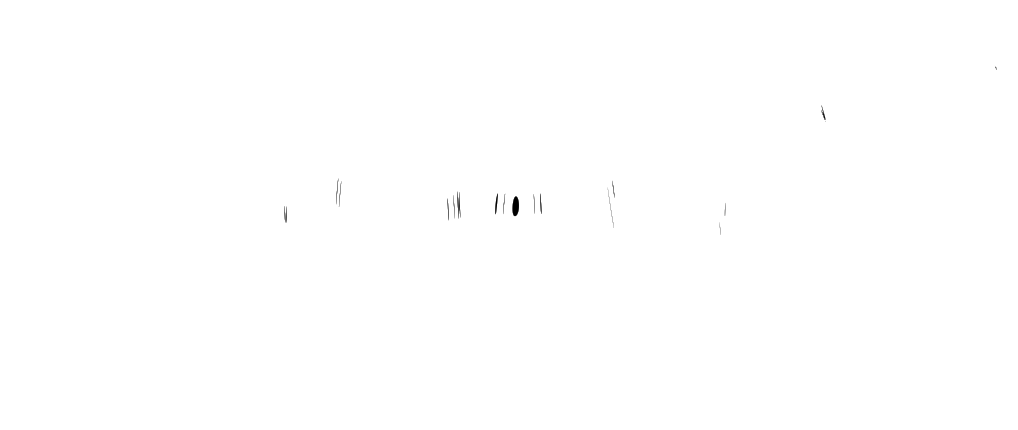
\includegraphics[width=3.5in]{image86r.png}}
\caption{Simulated scattering image of the pulsar.  The pulsar is
  modeled as a unit disk, with a much exagerated scale.  Flux
  conservation requires that the sum of image areas equals the
  original disk.
This compares favourably with the VLBI images of Brisken et al.~(2010)
}
\label{fig:2d}
\end{figure}

\section{Future Potential}

In our picture, pulsar scintillation is dominated by a small number of
magnetic discontinuities highly aligned to the line of sight.  Surface
waves will move very slowly in this projected geometry, allowing for a
precise determination of the geometric properties.  This allows the
use of these sheets as lenses to study both pulsars and the ISM.  

\subsection{ISM dynamics}

Free parameters in our model include the thickness of the sheet and the
inclination angle.  These can be inferred by broad band measurements
of pulsar scintillation, as follows. Firstly, the apparent position of images is expected to shift by
a distance of order of the sheet width, as one decreases the observing frequency from the
highest critical frequency at which the image forms, to a factor of
two below.  Secondly, the co-linearity of the images is related to
the inclination angle of the sheet: the more aligned is the sheet with the line of
sight, the greater is the aspect ratio of the scattering image.

\subsection{Pulsar Emission imaging}

A straightforward application is the study of the reflex motion of the
emission region of the pulsar across the pulse phase.  One expects the
apparent emission region to move by distance of order of the effective
emission height multiplied by the ratio of the pulse width to the
rotation period.  Using VLBI mapping of the scattering geometry, one
can precisely predict the change of scintillation pattern as a
function of pulse phase.  The effective astrometric precision can be
sub nano arcsecond.

\subsection{Distance Measurement}

It is tempting to use these lenses to obtain precision parallax
distances to pulsars.  
The challenges is to keep the lens stable over a year, when
typical pulsars move by much more than an astronomical unit, making
the differential measurements challenging.  In the sheet lensing
scenario, one can imagine obtaining widely separated scattering images:
the lensing angle scales as $\propto \lambda^2$, so at low
frequencies, for example with LOFAR LBA, hundreds of AU are probed.
Over the course of a year, persistent images should remain visible, and the
interference pattern could be studied as a function of annual
modulation.  This would result in direct parallax distances with nano arc
second precision, enough to determine pulsar distances for coherent
gravitational wave detection \citep{2010arXiv1010.4337B}.

\section{Conclusions}

We have presented a quantitative theory of pulsar scintillation
inverse parabolic arcs.  These extend recent ideas of
\citet{2006ApJ...640L.159G} and \citet{2012MNRAS.421L.132P} about thin
current sheets as the scattering objects in the ISM, which naturally
explain the large angle scattering observed in pulsars and some
extragalactic sources.

This picture could explain all scintillation phenomena from refractive
lensing, all with structures greater than 0.1 AU.  The apparent
diffractive structure results from the interference between refractive
images, and no diffractive scattering is needed.

In this scenario, VLBI monitoring of pulsars on time scales of weeks,
at multiple low frequencies, can allow forecasts of the scattering
behaviour.  This in turn could improve gravity wave timing residuals.
The same scenario also enables the coherent use of the scattered
images as a gigantic interstellar interferometer to map the motions of
the pulsar emission regions.

\section{Acknowledgements}

U-LP thanks NSERC and CAASTRO for support. YL is supported 
by the Australian Research Counsil Future Fellowship.


\newcommand{\araa}{ARA\&A}   % Annual Review of Astronomy and Astrophys.
\newcommand{\afz}{Afz}       % Astrofizica
\newcommand{\aj}{AJ}         % Astronomical Journal
\newcommand{\azh}{AZh}       % Astronomicekij Zhurnal
\newcommand{\aaa}{A\&A}      % Astronomy and Astrophysics
\newcommand{\aas}{A\&AS}     % Astronomy and Astrophys. Supplement Series
\newcommand{\aar}{A\&AR}     % Astronomy and Astrophysics Review
\newcommand{\apj}{ApJ}       % Astrophysical Journal
\newcommand{\apjs}{ApJS}     % Astrophysical Journal Supplement Series
\newcommand{\apjl}{ApJ}      % Astrophysical Journal Letters
\newcommand{\apss}{Ap\&SS}   % Astrophysics and Space Science
\newcommand{\baas}{BAAS}     % Bulletin of the American Astron. Society
\newcommand{\jaa}{JA\&A}     % Journal of Astronomy and Astrophysics
\newcommand{\mnras}{MNRAS}   % Monthly Notices of the Roy. Astron. Society
\newcommand{\nat}{Nat}       % Nature
\newcommand{\pasj}{PASJ}     % Publ. of the Astron. Society of Japan
\newcommand{\pasp}{PASP}     % Publ. of the Astron. Society of the Pacific
\newcommand{\paspc}{PASPC}   % Publ. Astron. Soc. Pacific Conf. Proc.
\newcommand{\qjras}{QJRAS}   % Quart. Journal of the Royal Astron. Society
\newcommand{\sci}{Sci}       % Science
\newcommand{\solphys}{Solar Physics}       % 
\newcommand{\sova}{SvA}      % Soviet Astronomy
\newcommand{\aap}{A\&A}


\bibliography{swave}
\bibliographystyle{mn2e}


\label{lastpage}

\end{document}
% ion gyromagnetic radius:
% m_p v^2/r = e v x B
% v=10^4 m/s, m_p = 1.7e-27 kg, e=1.6e-19C, B=1\mu G = 1e-10T
% r=m v/(eB) = 1.e6 m 
